\documentclass[letterpaper,10pt]{article}

\usepackage{enumitem}
\usepackage{titling}
\usepackage{listings}
\usepackage{url}
\usepackage{hyperref}
\usepackage{setspace}
\usepackage{subfig}
\usepackage{sectsty}
\usepackage{pdfpages}
\usepackage{colortbl}
\usepackage{multirow}
\usepackage{multicol}
\usepackage{relsize}
\usepackage{amsmath}
\usepackage{wasysym}
\usepackage{fancyvrb}
\usepackage[yyyymmdd]{datetime}
\usepackage{amsmath,amssymb,amsthm,graphicx,xspace}
\usepackage[titlenotnumbered,noend,noline]{algorithm2e}
\usepackage[compact]{titlesec}
\usepackage{XCharter}
\usepackage[T1]{fontenc}
\usepackage[scaled]{beramono}
\usepackage[normalem]{ulem}
\usepackage{booktabs}
\usepackage{tikz}
\usetikzlibrary{arrows,automata,shapes,trees,matrix,chains,scopes,positioning,calc}
\tikzstyle{block} = [rectangle, draw, fill=blue!20,
text width=2.5em, text centered, rounded corners, minimum height=2em]
\tikzstyle{bw} = [rectangle, draw, fill=blue!20,
text width=4em, text centered, rounded corners, minimum height=2em]

\definecolor{namerow}{cmyk}{.40,.40,.40,.40}
\definecolor{namecol}{cmyk}{.40,.40,.40,.40}
\renewcommand{\dateseparator}{-}

\let\LaTeXtitle\title
\renewcommand{\title}[1]{\LaTeXtitle{\textsf{#1}}}

\lstset{basicstyle=\footnotesize\ttfamily,breaklines=true}

\newcommand{\handout}[5]{
	\noindent
	\begin{center}
		\framebox{
			\vbox{
				\hbox to 5.78in { {\bf ECE 350: Real-Time Operating Systems } \hfill #2 }
				\vspace{4mm}
				\hbox to 5.78in { {\Large \hfill #4  \hfill} }
				\vspace{2mm}
				\hbox to 5.78in { {\em #3 \hfill \today} }
			}
		}
	\end{center}
	\vspace*{4mm}
}

\newcommand{\lecture}[3]{\handout{#1}{#2}{#3}{Lecture#1}}
\newcommand{\tuple}[1]{\ensuremath{\left\langle #1 \right\rangle}\xspace}

\newcommand{\Rplus}{\protect\hspace{-.1em}\protect\raisebox{.35ex}{\smaller{\smaller\textbf{+}}}}
\newcommand{\Cpp}{\mbox{C\Rplus\Rplus}\xspace}


\addtolength{\oddsidemargin}{-1.000in}
\addtolength{\evensidemargin}{-0.500in}
\addtolength{\textwidth}{2.0in}
\addtolength{\topmargin}{-1.000in}
\addtolength{\textheight}{1.75in}
\addtolength{\parskip}{\baselineskip}
\setlength{\parindent}{0in}
\renewcommand{\baselinestretch}{1.5}
\newcommand{\term}{Spring 2023}
\newcommand{\termnumeric}{1235}

\singlespace


\begin{document}

\lecture{ 17 --- Scheduling in Windows \& UNIX }{\term}{Jeff Zarnett}

\section*{Commercial OS Scheduling Algorithms}

In this section we will examine how real commercial operating systems schedule their processes and threads. We will examine UNIX, Windows, and finally, Linux scheduling. We will see what approaches are used and what is interesting or novel about them.

\subsection*{Traditional UNIX}

The traditional UNIX scheduling is really ancient; as in System V R3 and BSD 4.3. It was replaced in SVR4 (which had some real-time support). The information about the traditional UNIX scheduler comes primarily from~\cite{osi}.

The routine is a multilevel feedback system using Round Robin within each of the priority queues. Time slicing is implemented and the default time slice is a (very long) 1 second. So if a process does not block or complete within 1~s, then it will be preempted. Priority is based on the process type as well as the execution history.

Processor utilization for a process $j$ is calculated for an interval $i$ by the following formula:

\begin{center}
$CPU_{j}(i) = \dfrac{CPU_{j}(i - 1)}{2}$
\end{center}

And the priority is for process $j$ at interval $i$ is calculated by the formula:

\begin{center}
$P_{j}(i) = B_{j} + \dfrac{CPU_{j}}{2} + N_{j}$
\end{center}

where $B_{j}$ is the base priority of process $j$ and $N_{j}$ is the ``nice'' value of process $j$. The ``nice'' value is a UNIX way to allow a user to voluntarily reduce the priority of a process to be ``nice'' to other users (but honestly, who uses this?)~\cite{mos}. Actually, the answer to that question is: system administrators. An admin can ``re-nice'' a process and make it somewhat nicer than it would otherwise be.

The $CPU$ and $N$ components of the equation are restricted to prevent a process from migrating outside of its assigned category. A process is assigned to a given category based on what kind of process it is. To put it in simple terms, the OS puts its own needs first and tries to make the best use of resources it can. From highest to lowest priority, the categories are:

\begin{enumerate}
	\item Swapper (move processes to and from disk)
	\item Block I/O device control (e.g., disk)
	\item File manipulation
	\item Character I/O device control (e.g., keyboard)
	\item User processes
\end{enumerate}

Yes, unfortunately, user processes get piled at the bottom of the list. The use of the hierarchy should provide for efficient use of I/O devices and tends to penalize processor-bound processes at the expense of I/O bound processes. This is beneficial, because CPU-bound processes should be able to carry on executing when an I/O-bound process waits for the I/O operation to complete, but when an I/O operation is finished, we would like to start the next I/O operation so the I/O device is not waiting. This strategy is reasonably effective for a general-purpose, time-sharing operating system.

\subsection*{Windows}

Windows schedules threads using a priority-based, preemptive scheduling algorithm, ensuring that the highest priority thread runs. The official name for the selection routine is the \textit{dispatcher}. A thread will run until it is preempted, blocks, terminates, or until its time slice expires. If a higher priority thread is unblocked, it will preempt a lower priority thread. Windows has 32 different priority levels, the regular (priority 1 to 15) and real-time classes (16 to 31). A memory management task runs at priority 0. The dispatcher maintains a queue for each of the scheduling priorities and goes through them from highest to lowest (yes, in Windows, higher numbers are higher priorities) until it finds something to do (and if there is nothing else currently ready, the System Idle Process will ``run'')~\cite{osc}.

There are six priority classes you can set a process to via Task Manager, from highest to lowest:
\begin{enumerate}
	\item Realtime
	\item High
	\item Above Normal
	\item Normal
	\item Below Normal
	\item Low
\end{enumerate}

A process is usually in the Normal class. Within that class there are some more relative priorities. Unless it is in the real-time category, the relative priority can change. The details are summarized in the table below:

\begin{center}
	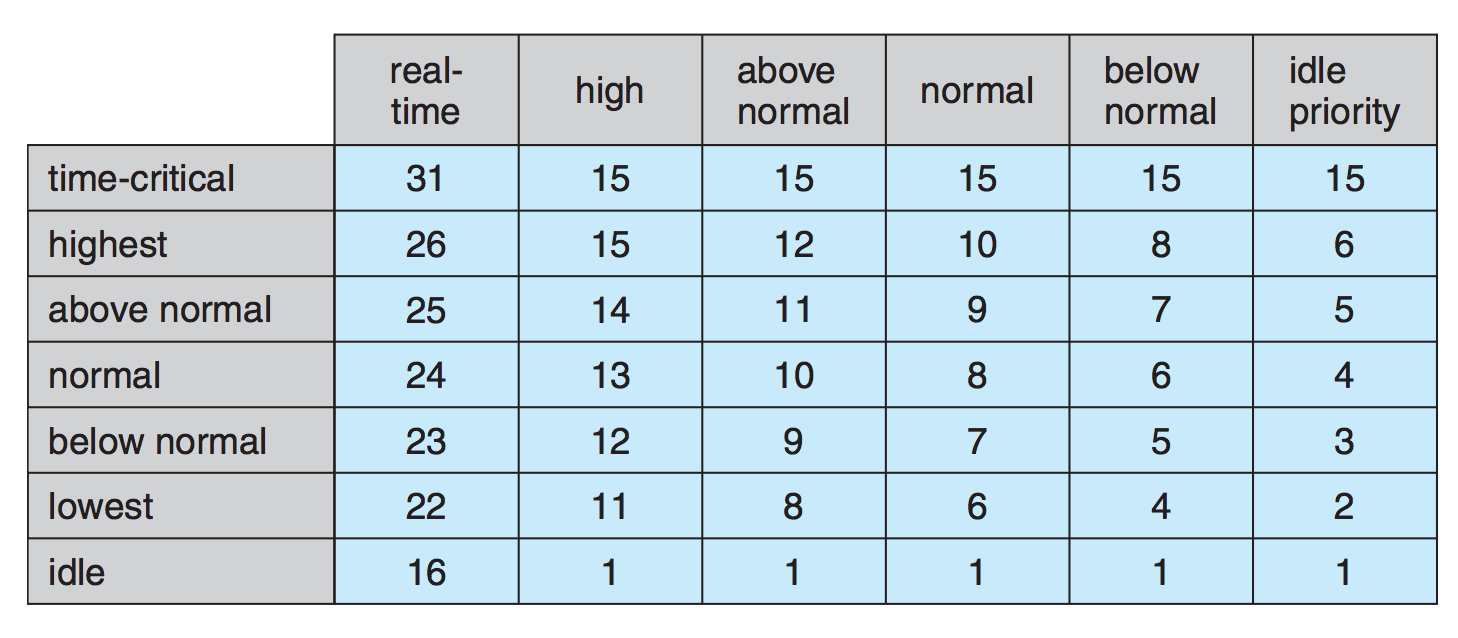
\includegraphics[width=0.7\textwidth]{images/windows-thread-priorities.png}\\
	Windows thread priorities~\cite{osc}.
\end{center}

If a process reaches the end of a time slice, the thread is interrupted, and unless it is in the real-time category, its priority will be lowered, to a minimum of a of the base priority of each class. When a process that was blocked on something (e.g., a wait or I/O), its priority is temporarily boosted (unless it is real-time, in which case it cannot be boosted). The amount of the boost depends on what the event was: a process that was waiting for keyboard input gets a bigger boost than one that was waiting for a disk operation, for example~\cite{osc}. 

The operating system also gives a priority to whatever process is running in the selected foreground window. This is different from foreground vs. background processes as discussed earlier, because the definition of a foreground process was one that was user-interactive. Here, the distinction is which of the user-interactive processes is currently ``on top'' in the UI. Not only does this process get a priority boost, but it also gets longer time slices. This can be disabled, if so desired, but it really highlights the different heritages of Windows and UNIX. UNIX was originally a time-sharing system with multiple users and lots of processes; Windows was originally a single-user desktop operating system doing one or maybe a few things at a time.


\bibliographystyle{alphaurl}
\bibliography{350}


\end{document}